% Crucial Preamble
\documentclass[12pt,letterpaper]{article} \usepackage{amsmath} \usepackage{graphicx} \usepackage[margin=1in]{geometry} \usepackage{longtable}  \usepackage{amssymb}

% Extra Preamble
\usepackage{fancyhdr} \usepackage{enumitem} \usepackage{float} \usepackage{soul}
\usepackage{multicol} \usepackage[compact]{titlesec}


% frames with display breaks
\usepackage{mdframed}
\allowdisplaybreaks

% change spacing
\usepackage{setspace}
\setlength{\parskip}{0.4\baselineskip}

% Remove paragraph indentation
\setlength{\parindent}{0pt}

% Reduce space before and after section headings
%\titlespacing*{\section}{0pt}{0.1\baselineskip}{0.2\baselineskip}

% changes font
%\renewcommand{\familydefault}{\sfdefault}

% adds header and footer
\pagestyle{fancy}
\fancyhead{} \fancyhead[C]{PHY 2323 Cheat Sheet} \fancyhead[L]{PHY2323} \fancyhead[R]{Owen Daigle}
\fancyfoot{} \fancyfoot[C]{\thepage}


\begin{document}
	
	\begin{center}
		\Large\textbf{PHY 2323 Cheat Sheet} \\
		\vspace{0.5em}
	\end{center}
	
	\section{Coordinate Systems}
	There are 3 main coordinate systems:
	\begin{enumerate}[]
		\item Cartesian ($x,y,z$)
		\item Cylindrical ($\rho, \phi, z$)
		\item Spherical ($r,\phi, \theta$)
	\end{enumerate}
	
	\section{Electric Fields}
	
	\subsection{Coulombs Law}
	Coulomb's law is used to sum up all the charges in a location which will give an electric field $E$.
	\begin{align*}
		\vec E (\vec r) = \frac{1}{4\pi \epsilon_0} \int_S \frac{\rho(\vec r\prime)(\vec r - \vec r\prime)}{|\vec r - \vec r\prime | ^3}\mathrm d l
	\end{align*}
	This can also be extended to a surface with $\mathrm ds$ and 2 integrals, or volume with $\mathrm dv$
	
	Note that anything with the $\prime$ means that it is related to the \textbf{surface of charge}, and anything without the prime is related to the \textbf{observation point.}
	
	\subsection{Gausses Law}
	Gausses Law can be used on a \textbf{closed surface} where we make a guassian surface (such as a sphere, or cylander) at the point of interest. 
	\begin{align*}
		\int_S \vec E \mathrm d \vec s = \frac{Q_{enc}}{\epsilon}
	\end{align*}

	We also have the $\vec D$ field which is the \textit{Electric Flux Density}.
	\begin{align*}
		\int_S \vec D \mathrm d \vec s = Q_{enc}
	\end{align*}
	
	Finally, we have the flux $\psi$, a scalar. 
	\begin{align*}
		\psi = \epsilon \int_s \vec E \mathrm d \vec s = \int \vec D \mathrm d \vec s
	\end{align*}

	This is useful in 3 main cases. 
	\begin{enumerate}[]
		\item Spherical Symmetry is present
		\item Cylindrical symmetry is present (long line of charge with uniform $\rho$ or cylander with no angular dependance)
		\item Planar Symmetry (Long 2D surface of charge)
	\end{enumerate}

	A useful piece of information is if we want to find the $Q_{enc}$, we can often just integrate the charge density in a volume $V$.
	\begin{align*}
		Q_{enc} = \iiint_V \rho \mathrm d V
	\end{align*}

	Also, the $\vec D$ field is just the $\vec E$ field times a factor of $\epsilon$ ($\vec D = \epsilon \vec E$) 
	
	\subsection{Energy Stored in an Electric Field}
	We say that $W$ is the energy stored in an electric field, or the energy required to assemble a charge distribution. 
	
	We can calculate this by summing up the product of the charge density and potential difference across a line/surface/volume.
	\begin{align*}
		W = \frac{1}{2}\int_{S\prime}\rho_s(\vec r\prime)*V(\vec r\prime) \mathrm d v\prime
	\end{align*}
	
	\section{Electric Potential}
	This is the potential energy per unit charge. AKA the voltage. This is a \textbf{scalar field}. This is \textit{independant of the path chosen}. 
	\begin{align*}
		V(\vec r) = \frac{1}{4\pi \epsilon _0} \int_{l\prime }\frac{\rho _l \mathrm d l\prime}{|\vec r-\vec r\prime| }
	\end{align*}
	This can be extended into 2d or 3d space by changing the $l\prime$ and $\mathrm d l\prime$ for $s\prime, \mathrm d s\prime$ or $v\prime, \mathrm d v\prime$.
	
	Then we can relate the change in voltage to the electric field:
	\begin{align*}
		\vec E = -\nabla V \qquad \nabla V = -\int \vec E\cdot \mathrm d \vec l
	\end{align*}

	\subsection{Electric Dipole}
	A \textbf{dipole} is a pair of equal and opposite charges that are very close to each other relative to the point of observation.
	
	This means that at the point of observation, they seem as one charge. 
	
	We have an equation that relates the charge of each end of the dipole $q$, the distance between the charges $d$, and the vector between the dipole and the observation point $\vec r$. This vector must be large compared to $d$.
	\begin{align*}
		V(\vec r) = \frac{(qd) \hat z \cdot \hat r}{4\pi \epsilon |r|^2}
	\end{align*}

	\subsection{Capacitors}
	The capacitence $C$ can be calculated using the following formula:
	\begin{align*}
		C=\frac{Q}{\Delta V}
	\end{align*}
	In practice, we use the following 3 step procedure:
	\begin{enumerate}[noitemsep]
		\item Find $E$
		\item Find $\Delta V$
		\item Find $C$ using $C=\frac{Q}{\Delta V} $
	\end{enumerate}
	
	\section{Materials in Electric Fields}
	There are 3 types of materials:
	\begin{enumerate}[]
		\item Conductors
		\item Insulators
		\item Semiconductors
	\end{enumerate}

	We have rules concerning the normal and tangential part of the boundary between 2 materials. 
	
	To obtain the normal part, we take the unit vector of the boundary, and this is our normal vector ($\hat n = \frac{\vec n}{|n|}$).
	
	If we then want to get the \textbf{normal part} of $E$, we dot product it with $\hat n$, then append $n$ to keep direction ($\vec E_n = (\vec E\cdot \hat n)\hat n$)
	
	The \textbf{tangential part }is just $\vec E_t = \vec E - \vec E_n$

	\subsection{Boundary between 2 Dielectrics}
	If we have 2 electric fields between 2 \textbf{dielectric} (insulators) surfaces, we have the following formulas for the bounds:
	\begin{align*}
		E_{1t} = E_{2t} \qquad \epsilon_1E_{1n}-\epsilon_2 E_{2n} = \rho_s
	\end{align*}

	\subsection{Surface of a Conductor}
	If we have an electric field at the \textbf{surface }of a \textbf{conductive} surface (note that inside the surface $E=0$), we have the following formulas for the bounds:
	\begin{align*}
		E_{1t} = E_{2t} = 0 \qquad E_{n} = \frac{\rho_s}{\epsilon_0}
	\end{align*}

	\section{Laplace and Poisson Equations}
	These equations will give us a general form of the equation for the solution, and then using 2 conditions (such as points) we can sub them into the form of the equation and solve the equation. 
	
	The whole laplacian equation is very complicated, but we have 2 special cases of note:
	\begin{align*}
		\nabla^2 V = \frac{-\rho_v}{\epsilon} \qquad \text{ or if no charge density (charges on surface): } \nabla^2V=0
	\end{align*}

	\begin{mdframed}
		\textbf{Ex. } As a very general example, if we want to find the voltage in a conductor (charges just on surface)
		
		We start by using the laplace equation:
		\begin{align*}
			\nabla^2 V = 0 \implies \frac{\partial^2 V}{\partial x^2} + \frac{\partial^2 V}{\partial y^2} + \frac{\partial^2 V}{\partial z^2} = 0
		\end{align*}
		\textit{For simplicity, I will consider a situation where the V only exists in the $z$ direction, hence the $x$ and $y$ components will be 0.}
		\begin{align*}
			\frac{\partial^2 V}{\partial z^2} = 0
		\end{align*}
		Since $\frac{\partial^2 V}{\partial z^2}=0$, then we must say that $\frac{\partial V}{\partial z} = a$ where $a$ is a constant. We must then say that $V = az+b$ where $a$ and $b$ are constants.
		
		This is because integrating $\frac{\partial^2 V}{\partial z^2}=0$ once gives us $\frac{\partial V}{\partial z}=a$ and then $a$ second time gives $V=az+b$
		
		Then we must have some boundary conditions given such as when $z=0$, $V=0$, and when $z=1$, $V=5$. Then we can sub in and solve for $a$ and $b$.
		
		Then we have $V$ at any point.
	\end{mdframed}

	We can also do this for spherical or cylindrical coordinates, except for the laplacian ($\nabla^2$) is different.
	
	\section{Currents}
	Current is just the rate of which charge travels with respect to time. Measured in either $\frac{C}{s}$ or $A$.
	
	By definition, the current density is just the amount of current passing through a cross sectional area. Note that this does NOT include parallel current since this current does not actually traverse \textbf{through} the cross sectional area.
	\begin{align*}
		\vec J=\frac{I}{A} \qquad I = \int_S \vec J \cdot \mathrm d \vec s
	\end{align*}

	\subsection{Resistance}
	Resistance is defined as:
	\begin{align*}
		R = \frac{L}{\sigma A} = \frac{\rho L}{A}
	\end{align*}
	These are equivalent since $\sigma = \rho^{-1}$ where $\rho$ is the resistivity, and $\sigma$ is the conductivity.
	
	Those equations work fine for a single area, but if we need to sum up the areas, we have 2 techniques. The first is just by summing up the above equation. The second is based on Ohms law. 
	\begin{align*}
		 R = \frac{L}{\sigma A} = \int_l \frac{\mathrm d \vec l}{\iint_S \sigma \mathrm d \vec s} \qquad R = \frac{\Delta V}{I} = \frac{-\int_l \vec E \cdot \mathrm d \vec l}{\int_S \vec J \cdot \mathrm d \vec s} 
	\end{align*}

	\begin{mdframed}
		\textbf{Ex. }
	\end{mdframed}
	
	\subsection{Equation of Continuity}
	This basically says that if there is a current going out of an object, then there will be less charges in that object. 
	\begin{align*}
		\nabla \cdot \vec J = -\frac{\partial \rho_v}{\partial t}
	\end{align*}

	The relaxation time is the amount of time it takes for electrons to settle into their equilibrium. This ($\tau$) is: $\tau = \frac{\epsilon}{\sigma}$
	
	\section{Magnetic Fields}
	Similarly to electric fields, we have 2 fields seperated by a constant $\mu_0$. There is the $\vec B$ field (Magnetic Flux Density) and the $\vec H$ field (Magnetic Field). $\vec H = \ \frac{\vec B}{\mu_0}$
	
	\subsection{Biot-Savard}
	This law is how we calculate the magnetic field. This is similar to coulombs law (for electric fields) but for magnetic fields. Although, the versions for L, S, and V are slightly different (Line uses I, Surface and Sphere use $J_S$ and $J_V$.)
	\begin{align*}
		\vec B = \frac{\mu_0}{4\pi}\int_{l\prime}\frac{I\mathrm d \vec l\prime \times (\vec r - \vec r\prime)}{|\vec r - \vec r\prime |^3} \qquad \vec B = \frac{\mu_0}{4\pi}\int_{S\prime}\frac{J_s\mathrm \times (\vec r - \vec r\prime)d \vec S\prime}{|\vec r - \vec r\prime |^3} \qquad \vec B = \frac{\mu_0}{4\pi}\int_{V\prime}\frac{J_V\mathrm \times (\vec r - \vec r\prime)d \vec V\prime}{|\vec r - \vec r\prime |^3}
	\end{align*}

	We can use the right hand rule to see the direction of the generated field due to the cross product inside the calculation. 
	\begin{center}
		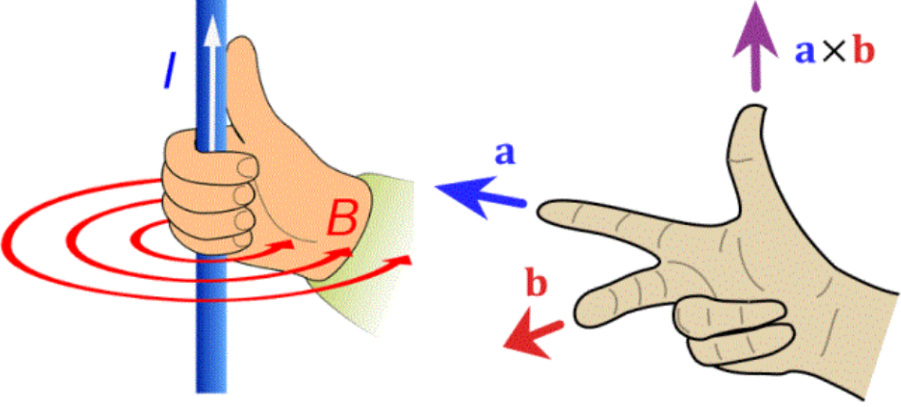
\includegraphics[width=0.7\linewidth]{rhr}
	\end{center}

	This direction will be perpendicular to both the current, and the $\vec r-\vec r\prime$ vector. 
	
	\subsection{Amperes Law}
	This is just like gausses law for electric fields in that it allows us to simplify the calculations for magnetic fields, but only under specific curcumstances. 
	
	Basically, we create an amperian loop (path) that when taken the dot product with the H field creates a nice math situation.
	\begin{align*}
		\oint \vec H \cdot \mathrm d \vec l = I_{enclosed}
	\end{align*}
	\begin{enumerate}[noitemsep]
		\item Predict Direction of $\vec H$
		\item Choose amperian path
		\item Calculate
	\end{enumerate}

	\subsection{Magnetic Forces}
	We say that the magnetic force produced by a wire 1 on another wire 2 is: 
	\begin{align*}
		\vec F_2 = \int I_2\mathrm d \vec l_2 \times \vec B_1
	\end{align*}
	So basically we need to get $\vec B$ using probably amperes law, and then assuming we know I, we can calculate the magnetic force $\vec F_m$.
	
	
	
	
	
\end{document}